\documentclass[a4paper, 11pt]{article}
\usepackage{amsmath, amssymb, amsthm}
\usepackage{graphicx}
\usepackage{float}
\usepackage{geometry}
\usepackage{booktabs}
\usepackage{caption}
\usepackage[colorlinks=true,linkcolor=blue,citecolor=blue,urlcolor=blue]{hyperref}
\geometry{margin=1in}
\newtheorem{theorem}{Theorem}
\newtheorem{lemma}{Lemma}
\title{Technical Documentation for CIFAR-10 Experiment}
\author{}
\date{}

\begin{document}

\maketitle

\section{Initial and Distilled Models}

This section describes the implementation, architecture, training process, and evaluation of both the initial and distilled models for CIFAR-10 classification.

\subsection{Model Architecture}

The architecture of both the initial and distilled models consists of a series of convolutional and fully connected layers, as summarized in Table~\ref{tab:architecture}. The design includes dropout layers for regularization and ReLU activation functions for non-linearity~\cite{krizhevsky2012imagenet}.

\begin{table}[H]
    \centering
    \caption{Overview of CIFAR-10 Model Architecture}
    \label{tab:architecture}
    \begin{tabular}{@{}ll@{}}
        \toprule
        \textbf{Layer Type} & \textbf{CIFAR-10 Architecture} \\
        \midrule
        ReLU Convolutional  & 64 filters (3x3) \\
        ReLU Convolutional  & 64 filters (3x3) \\
        Max Pooling         & 2x2 \\
        ReLU Convolutional  & 128 filters (3x3) \\
        ReLU Convolutional  & 128 filters (3x3) \\
        Max Pooling         & 2x2 \\
        ReLU Fully Connect. & 256 units \\
        ReLU Fully Connect. & 256 units \\
        Logits              & 10 units \\
        \bottomrule
    \end{tabular}
\end{table}

\subsection{Training Parameters}

The training parameters for the initial and distilled models are summarized in Table~\ref{tab:training_params}. Key differences include the learning rate, momentum schedule, and the addition of temperature scaling for the distilled model~\cite{papernot2016distillation}.

\begin{table}[H]
    \centering
    \caption{Training Parameters for Initial and Distilled Models}
    \label{tab:training_params}
    \begin{tabular}{@{}lll@{}}
        \toprule
        \textbf{Parameter} & \textbf{Initial Model} & \textbf{Distilled Model} \\
        \midrule
        Learning Rate       & 0.01 (decayed by 0.5 every 10 epochs) & 0.03 (decayed by 0.95 every 5 epochs) \\
        Momentum            & 0.9 (decayed by 0.5 every 10 epochs) & 0.9 (decayed by 0.8 every 10 epochs) \\
        Dropout Rate        & 0.5 & 0.5 \\
        Batch Size          & 128 & 128 \\
        Epochs              & 50 & 50 \\
        Weight Decay        & None & $1 \times 10^{-4}$ \\
        Temperature         & None & 5 \\
        Gradient Clipping   & None & 1.0 \\
        \bottomrule
    \end{tabular}
\end{table}

\subsection{Soft Label Generation}

Soft labels for the distilled dataset were generated using the softmax function with temperature scaling. The initial model produces raw logits as output, which are transformed into probabilities during the distillation process~\cite{papernot2016distillation}:
\begin{align*}
    \hat{y}_i = \frac{\exp\left(\frac{z_i}{T}\right)}{\sum_j \exp\left(\frac{z_j}{T}\right)},
\end{align*}
where $z_i$ represents the logits for class $i$ and $T = 5$ is the temperature.

\subsection{Theoretical Foundations and Techniques}

To enhance the performance and robustness of the models, several theoretical approaches and techniques were employed:
\begin{enumerate}
    \item \textbf{Weight Initialization:} Xavier initialization was used to ensure balanced variance across layers:
    \begin{align*}
        W \sim \mathcal{U}\left(-\sqrt{\frac{6}{n_{in} + n_{out}}}, \sqrt{\frac{6}{n_{in} + n_{out}}}\right),
    \end{align*}
    where $n_{in}$ and $n_{out}$ denote the number of input and output units~\cite{krizhevsky2012imagenet}.

    \item \textbf{KL Divergence Loss:} For the distilled model, knowledge transfer is achieved using Kullback-Leibler (KL) divergence~\cite{goodfellow2015explaining}:
    \begin{align*}
        D_{KL}(P \parallel Q) = \sum_i P_i \log \frac{P_i}{Q_i},
    \end{align*}
    where $P$ is the soft target distribution and $Q$ is the student model's output.
\end{enumerate}

\begin{figure}[H]
    \centering
    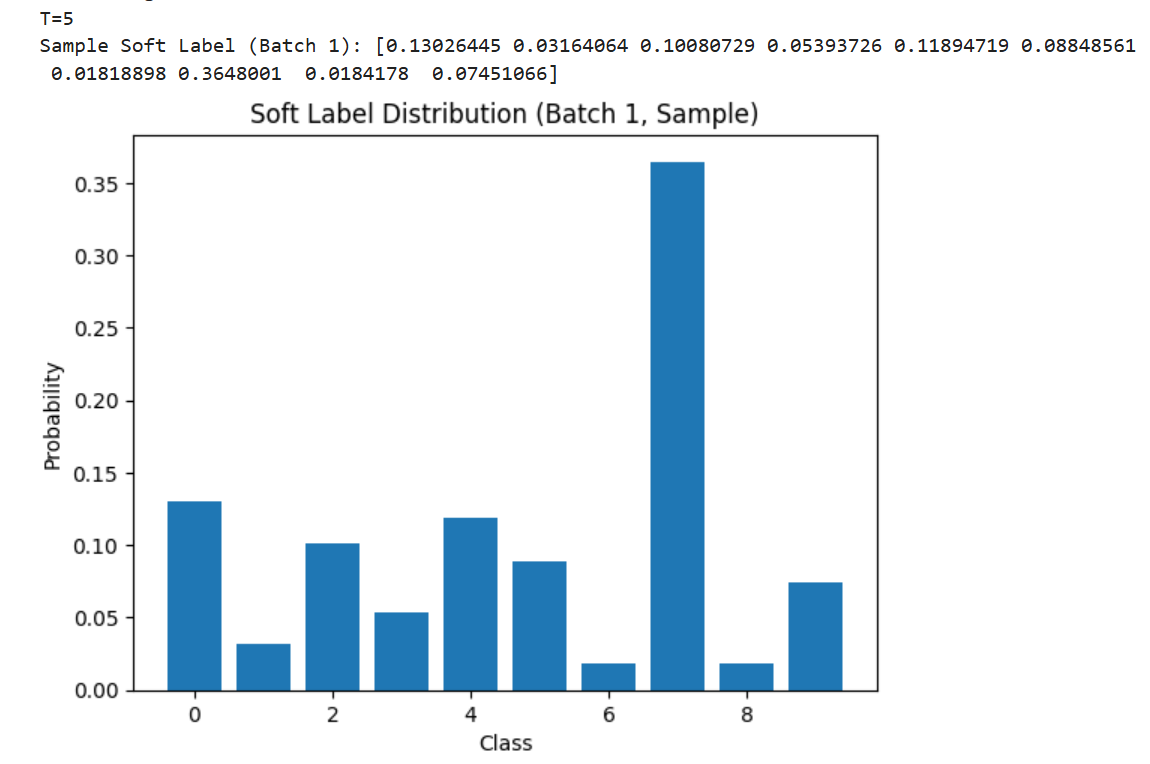
\includegraphics[width=0.8\textwidth]{soft_labels_sample.png}
    \caption{Sample Soft Label Distribution (T=5)}
    \label{fig:soft_labels}
\end{figure}


\subsection{Accuracy and Loss Analysis}

The performance of the initial and distilled models is shown in Figures~\ref{fig:test_accuracy_comparison} and~\ref{fig:train_loss_comparison}. These graphs illustrate the differences in test accuracy and training loss over epochs~\cite{szegedy2014intriguing}.

\begin{figure}[H]
    \centering
    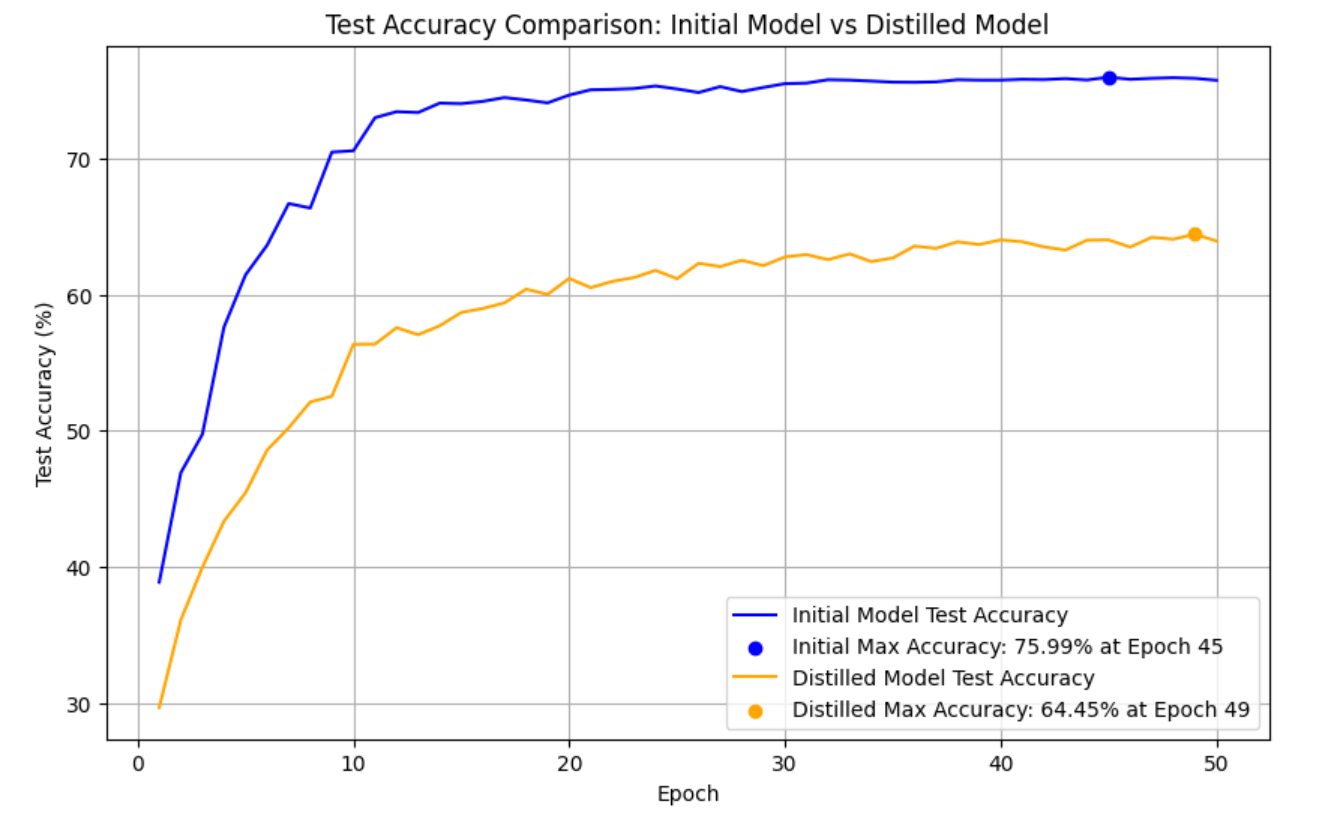
\includegraphics[width=0.8\textwidth]{test_accuracy_comparison.png}
    \caption{Test Accuracy Comparison: Initial Model vs Distilled Model}
    \label{fig:test_accuracy_comparison}
\end{figure}

\begin{figure}[H]
    \centering
    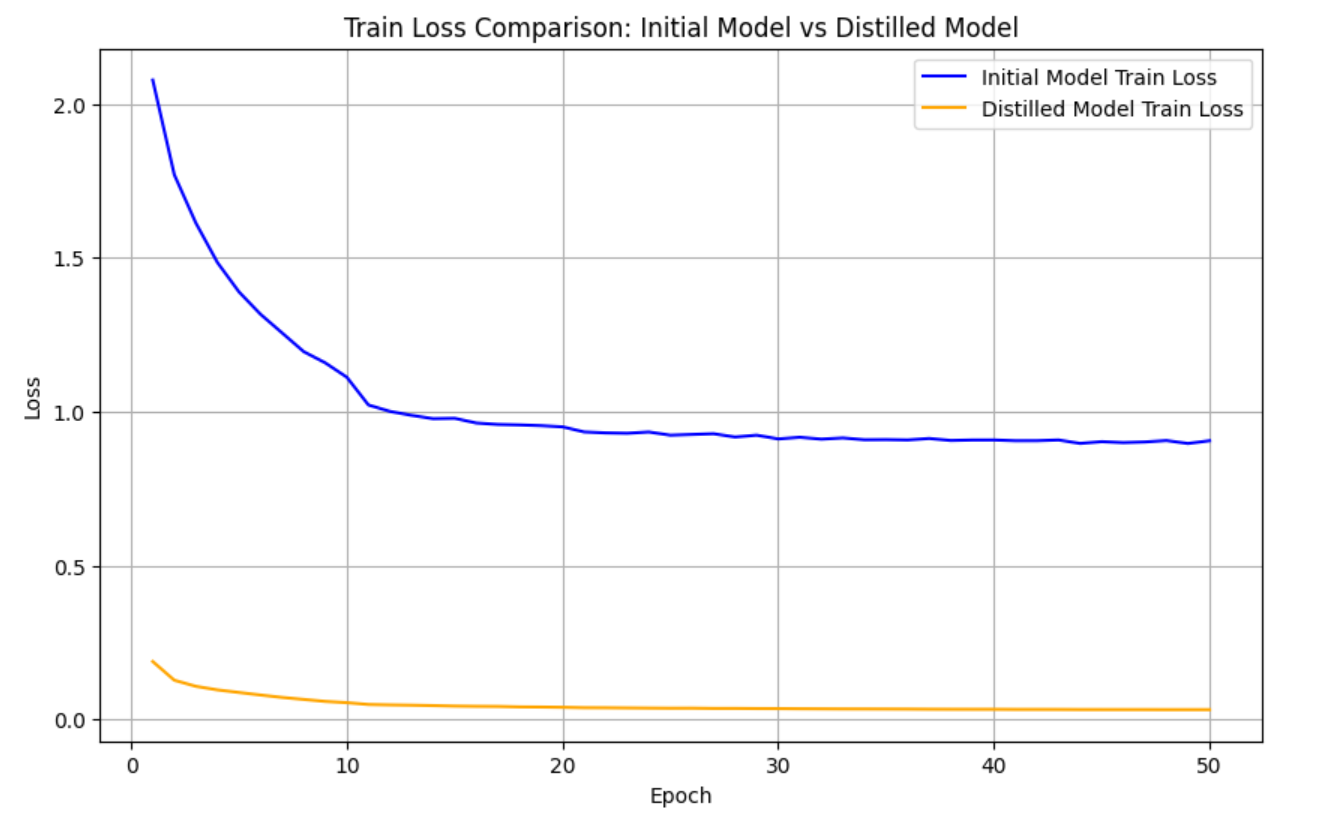
\includegraphics[width=0.8\textwidth]{train_loss_comparison.png}
    \caption{Train Loss Comparison: Initial Model vs Distilled Model}
    \label{fig:train_loss_comparison}
\end{figure}
\section{Robustness Evaluation}

This section evaluates the robustness of the initial and distilled models under adversarial attacks and varying temperature conditions.

\subsection{PGD Attack Configuration}

The adversarial samples were generated using the Projected Gradient Descent (PGD) method. The PGD algorithm iteratively refines adversarial examples by maximizing the loss function while keeping the perturbations within an $\epsilon$-ball :
\begin{align*}
    x_{t+1} = \Pi_{\mathcal{B}(x, \epsilon)} \left( x_t + \alpha \cdot \text{sign}\left( \nabla_x \mathcal{L}(x_t, y) \right) \right),
\end{align*}
where $\alpha$ is the step size, and $\Pi_{\mathcal{B}}$ projects the adversarial sample back into the $\epsilon$-ball around the original input.

\subsection{Theoretical Foundations}

\begin{theorem}[Lipschitz Continuity \cite{szegedy2014intriguing}]
    The robustness of a neural network to small perturbations can be analyzed using its Lipschitz constant $K$, defined as:
    \begin{align*}
        \|f(x_1) - f(x_2)\| \leq K \|x_1 - x_2\|.
    \end{align*}
    A smaller $K$ implies a more robust model.
\end{theorem}

\begin{lemma}[Adversarial Robustness Bound \cite{goodfellow2015explaining}]
    For any classifier $f$, the adversarial risk is bounded by:
    \begin{align*}
        \mathbb{P}(f(x + \delta) \neq y) \leq \exp\left(-\frac{\|\delta\|^2}{2\sigma^2}\right),
    \end{align*}
    where $\delta$ is the adversarial perturbation, and $\sigma$ is the standard deviation of the input noise.
\end{lemma}

\subsection{Attack Success Rates}

The attack success rates for both the initial and distilled models were evaluated and are visualized in Figures~\ref{fig:pgd_robustness}.
\begin{figure}[H]
    \centering
    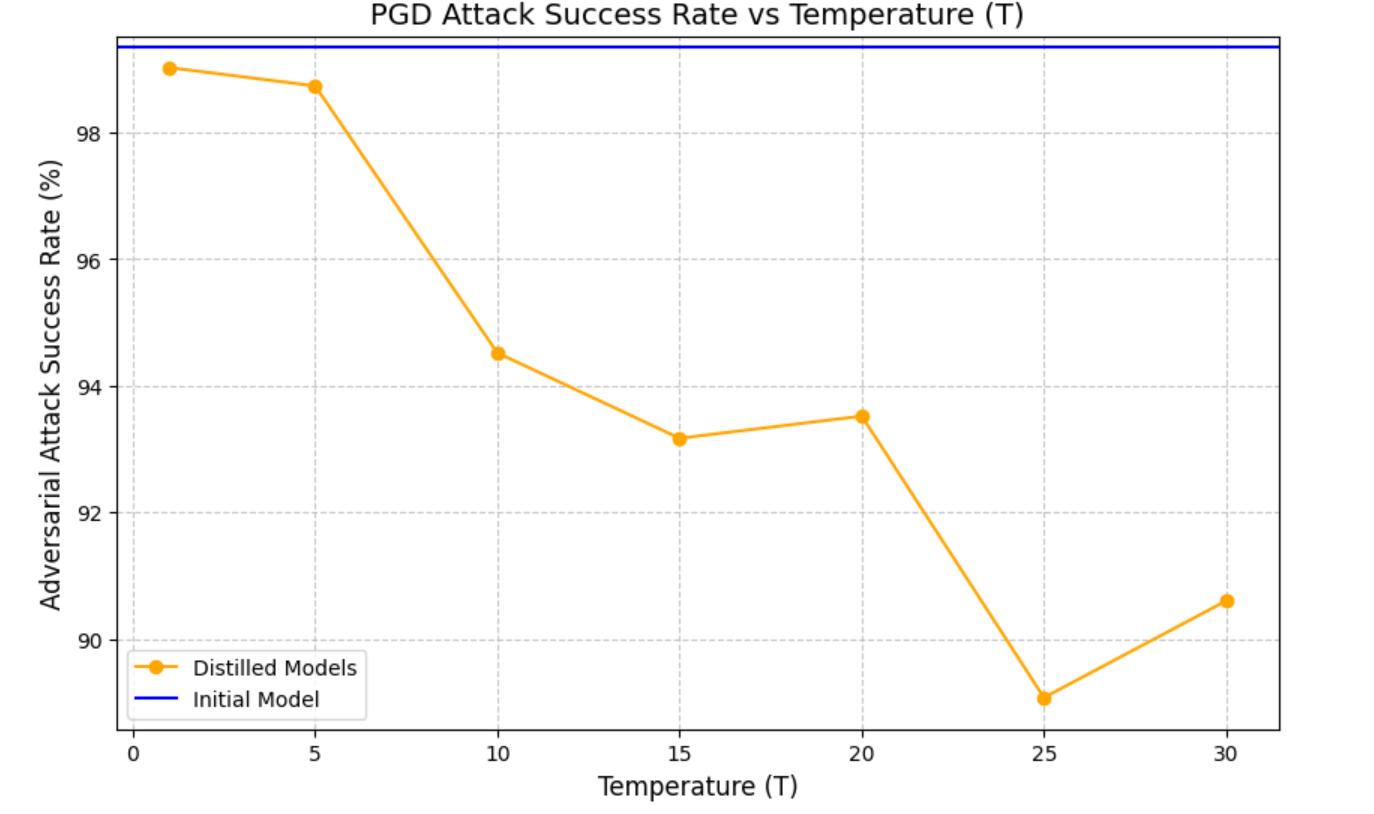
\includegraphics[width=0.8\textwidth]{pgd_robustness.png}
    \caption{PGD Attack Success Rate}
    \label{fig:pgd_robustness}
\end{figure}

The results indicate that the initial model achieves a PGD attack success rate of \textbf{99.36\%}. However, the distilled model demonstrates improved robustness, with reduced attack success rates as temperature increases.



\section{References}

\begin{thebibliography}{99}

\bibitem{krizhevsky2012imagenet}
A. Krizhevsky, I. Sutskever, and G. E. Hinton, 
"ImageNet classification with deep convolutional neural networks," 
\textit{Advances in Neural Information Processing Systems}, 2012, pp. 1097--1105.

\bibitem{papernot2016distillation}
N. Papernot, P. McDaniel, X. Wu, S. Jha, and A. Swami, 
"Distillation as a Defense to Adversarial Perturbations against Deep Neural Networks," 
\textit{IEEE Symposium on Security and Privacy}, 2016.

\bibitem{szegedy2014intriguing}
C. Szegedy, W. Zaremba, I. Sutskever, J. Bruna, D. Erhan, I. Goodfellow, and R. Fergus, 
"Intriguing properties of neural networks," 
\textit{International Conference on Learning Representations}, 2014.

\bibitem{goodfellow2015explaining}
I. J. Goodfellow, J. Shlens, and C. Szegedy, 
"Explaining and harnessing adversarial examples," 
\textit{International Conference on Learning Representations}, 2015.

\end{thebibliography}

\end{document}
